\documentclass[12pt]{article}

\usepackage{dsfont}
\usepackage{amsmath}
\usepackage{graphicx}
\usepackage[margin=1in]{geometry}

\usepackage{bm}
\newcommand{\m}[1]{\mathbf{\bm{#1}}}
\newcommand{\R}{I\hspace{-4.4pt}R}

\setlength\parindent{0pt}

\begin{document}

Mickey Warner

\subsection*{1. Prove the results about the smoothness of the members of the Mat{\'e}rn family.}

We use the theorem that if 
\[ \frac{d^{2\nu}}{d\tau^{2\nu}}\rho(\tau) \]
exists and is finite at $\tau=0$, then the random field having $\rho(\tau)$ as its correlation function is $\nu$ times differentiable at $0$.
\bigskip

Without loss of generality, let $\phi=1$. The Mat{\'e}rn correlation function is given by
\[ \rho(\tau) = \frac{\tau^\nu}{2^{\nu-1}\Gamma(\nu)}K_\nu(\tau),~~~~~~~~\tau\geq0,\nu>0. \]
For small $\tau$ and $\nu>0$, $K_\nu(\tau)\approx \Gamma(\nu)2^{\nu-1}\tau^{-\nu}$. Also, $\frac{d}{d\tau}\tau^\nu K_\nu(\tau)=-\tau^\nu K_{\nu-1}(\tau)$ and $K_\nu(\tau)=K_{-\nu}(\tau)$. We will be taking $\tau\rightarrow 0$, so we use the approximation for $K_\nu(\tau)$. This leads to the derivative,
\begin{align*}
\frac{d}{d\tau}\rho(\tau) &= -\frac{\tau^\nu}{2^{\nu-1}\Gamma(\nu)}K_{\nu-1}(\tau) \\
 &= \begin{cases} -\frac{\tau^\nu}{2^{\nu-1}\Gamma(\nu)}K_{\nu-1}(\tau),~~~~~&\nu-1\geq0 \\
 -\frac{\tau^\nu}{2^{\nu-1}\Gamma(\nu)}K_{1-\nu}(\tau),~~~~~&\nu-1<0 \end{cases} \\
 &\approx \begin{cases} -\frac{\tau^\nu}{2^{\nu-1}\Gamma(\nu)}\Gamma(\nu-1)2^{\nu-2}\tau^{-\nu+1},~~~~~&\nu-1\geq0 \\
 -\frac{\tau^\nu}{2^{\nu-1}\Gamma(\nu)}\Gamma(1-\nu)2^{-\nu}\tau^{\nu-1},~~~~~&\nu-1<0 \end{cases} \\
 &\approx \begin{cases} -\tau G_1(\nu),~~~~~&\nu-1\geq0 \\
 -\tau^{2\nu-1}G_2(\nu),~~~~~&\nu-1<0 \end{cases}. \\
\end{align*}
Therefore,
\begin{align*}
\rho'(0) &\begin{cases} =0,~~~~~&\nu\geq1 \\
 \in(-\infty,0),~~~~~&1/2\leq\nu<1  \\
 =-\infty,~~~~~&0<\nu<1/2 \end{cases}. \\
\end{align*}
The second derivative is given by
\begin{align*}
\rho''(\tau) &= \begin{cases} \frac{-\tau^{\nu-1} K_{\nu-1}(\tau)+\tau^\nu K_{\nu-2}(\tau)}{2^{\nu-1}\Gamma(\nu)},~~~~~ &\nu\geq2 \\
  \frac{-\tau^{\nu-1} K_{\nu-1}(\tau)+\tau^\nu K_{2-\nu}(\tau)}{2^{\nu-1}\Gamma(\nu)},~~~~~ &1\leq\nu<2 \\
  \frac{-\tau^{\nu-1} K_{1-\nu}(\tau)+\tau^\nu K_{2-\nu}(\tau)}{2^{\nu-1}\Gamma(\nu)},~~~~~ &0<\nu<1 
\end{cases}, \\
\end{align*}
and is evaluated at $\tau=0$ to
\begin{align*}
\rho''(0) \begin{cases} =0,~~~~~ &\nu\geq2 \\
  \in(-\infty,0),~~~~~ &1\leq\nu<2 \\
  =-\infty,~~~~~ &0<\nu<1 
\end{cases}. \\
\end{align*}
We have that the second derivative is finite when $\nu\geq 1$, leading to a random field that is one time mean square differentiable. To show this generalizes to $\nu\geq d$, we need to keep taking derivatives of $\rho(\tau)$. I suspect that on each even derivative, the orders of certain Bessel functions are negated when those orders are less than $\nu$. When this happens, the approximation will lead to a term having $\tau$ raised to a negative exponent causing the derivative to evaluate to $-\infty$.


\subsection*{2. Use the spectral representation to show that the product of two valid correlation functions is a valid correlation function.}

A valid correlation function is the characteristic function of some random variable,

\[ \rho(\m{\tau}) = E\left[e^{i\m{\tau}^\top\m{X}}\right]. \]

Suppose we have two valid correlation functions $\rho_1(\tau)$ and $\rho_2(\tau)$ associated with independent random variables $\m{X}_1$ and $\m{X}_2$, respectively. Then the product is written

\begin{align*}
\rho(\m{\tau}) = \rho_1(\m{\tau})\rho_2(\m{\tau}) &= E\left[e^{i\m{\tau}^\top\m{X}_1}\right]E\left[e^{i\m{\tau}^\top\m{X}_2}\right] \\
 &= E\left[e^{i\m{\tau}^\top\m{X}_1}e^{i\m{\tau}^\top\m{X}_2}\right] \\
 &= E\left[e^{i\m{\tau}^\top(\m{X}_1+\m{X}_2)}\right], 
\end{align*}

so $\rho$ is the characteristic function of $\m{X}_1+\m{X}_2$ and thus the product of two valid correlation functions is a valid correlation function. Note, our assumption of independence for $\m{X}_1$ and $\m{X}_2$ presents no issues. $\m{X}_1$ and $\m{X}_2$ may be dependent, but then we could simply define new independent random variables $\m{Y}_1$ and $\m{Y}_2$ with the same marginal distributions as $\m{X}_1$ and $\m{X}_2$, resulting in the same correlation functions in either case.

\subsection*{3. The spectral density of a correlation in the Mat{\'e}rn family has tails whose thickness depends on the smoothness parameter. Conjecture: the smoothness of the corresponding random field depends on the number of moments of the spectral density. What can you say about this conjecture?}

For correlation function

\[ \rho(\tau) \propto (a\tau)^\nu K_\nu(a\tau),~~~~~~~~\tau\geq0,\nu>0,a=1/\phi>0, \]
we have the corresponding spectral density
\[ f(x) \propto \frac{1}{\left(1+(x/a)^2\right)^{\nu+n/2}}, \]
where $n$ is the dimension $\tau$ (and $x$). This density has a form comparable to the $t$-distribution. Using integration by parts, we calculate the $k$th moment as
\begin{align*}
E(X^k) &\propto \int x^k(1+(x/a)^2)^{-(\nu+n/2)} dx \\
 &= \left.-\frac{a^2}{2\nu+n-2}\frac{x^{k-1}}{(1+(x/a)^2)^{(2\nu+n-2)/2}}\right\vert_{-\infty}^{\infty}+\int\frac{(k-1)a^2}{2\nu+n-2}\frac{x^{k-2}}{(1+(x/a)^2)^{-(2\nu+n-2)/2}} dx.
\end{align*}
The first term (and hence the second term also) will be finite when $2\nu+n-2\geq k-1$, or $\nu\geq(k-n+1)/2$. In one dimension, $n=1$, we see that when $\nu \geq k/2$ the $k$th moment exists. This may be related to the theorem used in the first problem, that we need to have $2d$-differentiable correlation function to have a $d$-differentiable random field. Here, we need the $2d$th moment to exist, i.e. $\nu\geq d$, to have smoothness.

\subsection*{4. Use the K-L representation to approximate the exponential correlation for range parameter equal to 1. Plot the approximation for several orders and compare to the actual correlation.}

The Karhunen-Loeve representation for a random process is given by
\[ X(s)=\sum_{j=1}^\infty\sqrt{\lambda_j}\psi_j(s)Z_j \]
where $Z_j$ are mean zero processes with $E(Z_jZ_k)=\delta_{jk}$ and $\psi_j$ is a basis of orthogonal functions such that
\[ \int\psi_j(s)\overline{\psi_k(s)}ds = \delta_{jk} \]
and
\[ \int C(s,s')\psi_j(s)ds=\lambda_j\psi_j(s'). \]
For an exponential correlation function with $\phi=1$ on an interval $[-L,L]$, we have
% \begin{align*}
% \lambda_{j1}=\frac{2}{w_{j1}^2+1}, & & \psi_{j1}=\frac{\cos(w_{j1}s)}{\sqrt{L+\sin(2w_{j1}L)/(2w_{j1})}} \\
% \lambda_{j2}=\frac{2}{w_{j2}^2+1}, & & \psi_{j2}=\frac{\sin(w_{j2}s)}{\sqrt{L-\sin(2w_{j2}L)/(2w_{j2})}} \\
% \end{align*}

\begin{align*}
\lambda_i = \begin{cases} 2/(1+v_j^2),~~~~~&i=2j+1 \\
 2/(1+w_k^2),~~~~~&i=2k \\
\end{cases} \\
\end{align*}

\begin{align*}
\psi_i(s) = \begin{cases} \frac{\cos(v_js)}{\sqrt{L+\sin(2v_jL)/(2v_j)}},~~~~~&i=2j+1 \\
 \frac{\sin(w_ks)}{\sqrt{L-\sin(2w_k}L)/(2w_k)},~~~~~&i=2k \\
\end{cases}, \\
\end{align*}
where $v_j$ and $w_k$ are the non-negative solutions to
\begin{align*}
1 - v\tan(vL) &= 0 \\
w + \tan(wL) &= 0 \\
\end{align*}
sorted in increasing order. We end the approximation at $J=5,10,20,50$ summands. We let $Z_j\sim N(0,1)$, $j=1,\ldots,J$ and $L=2\pi$ and obtain realizations of $X(s)$ on a grid $s\in[-4\pi, 4\pi]$. We also obtain realizations with \texttt{geoR}'s \texttt{grf()} function which produces realizations from a Gaussian process. One draw for each $J$ is shown (top four) and two Gaussian process draws are given (bottom two).

\begin{center}
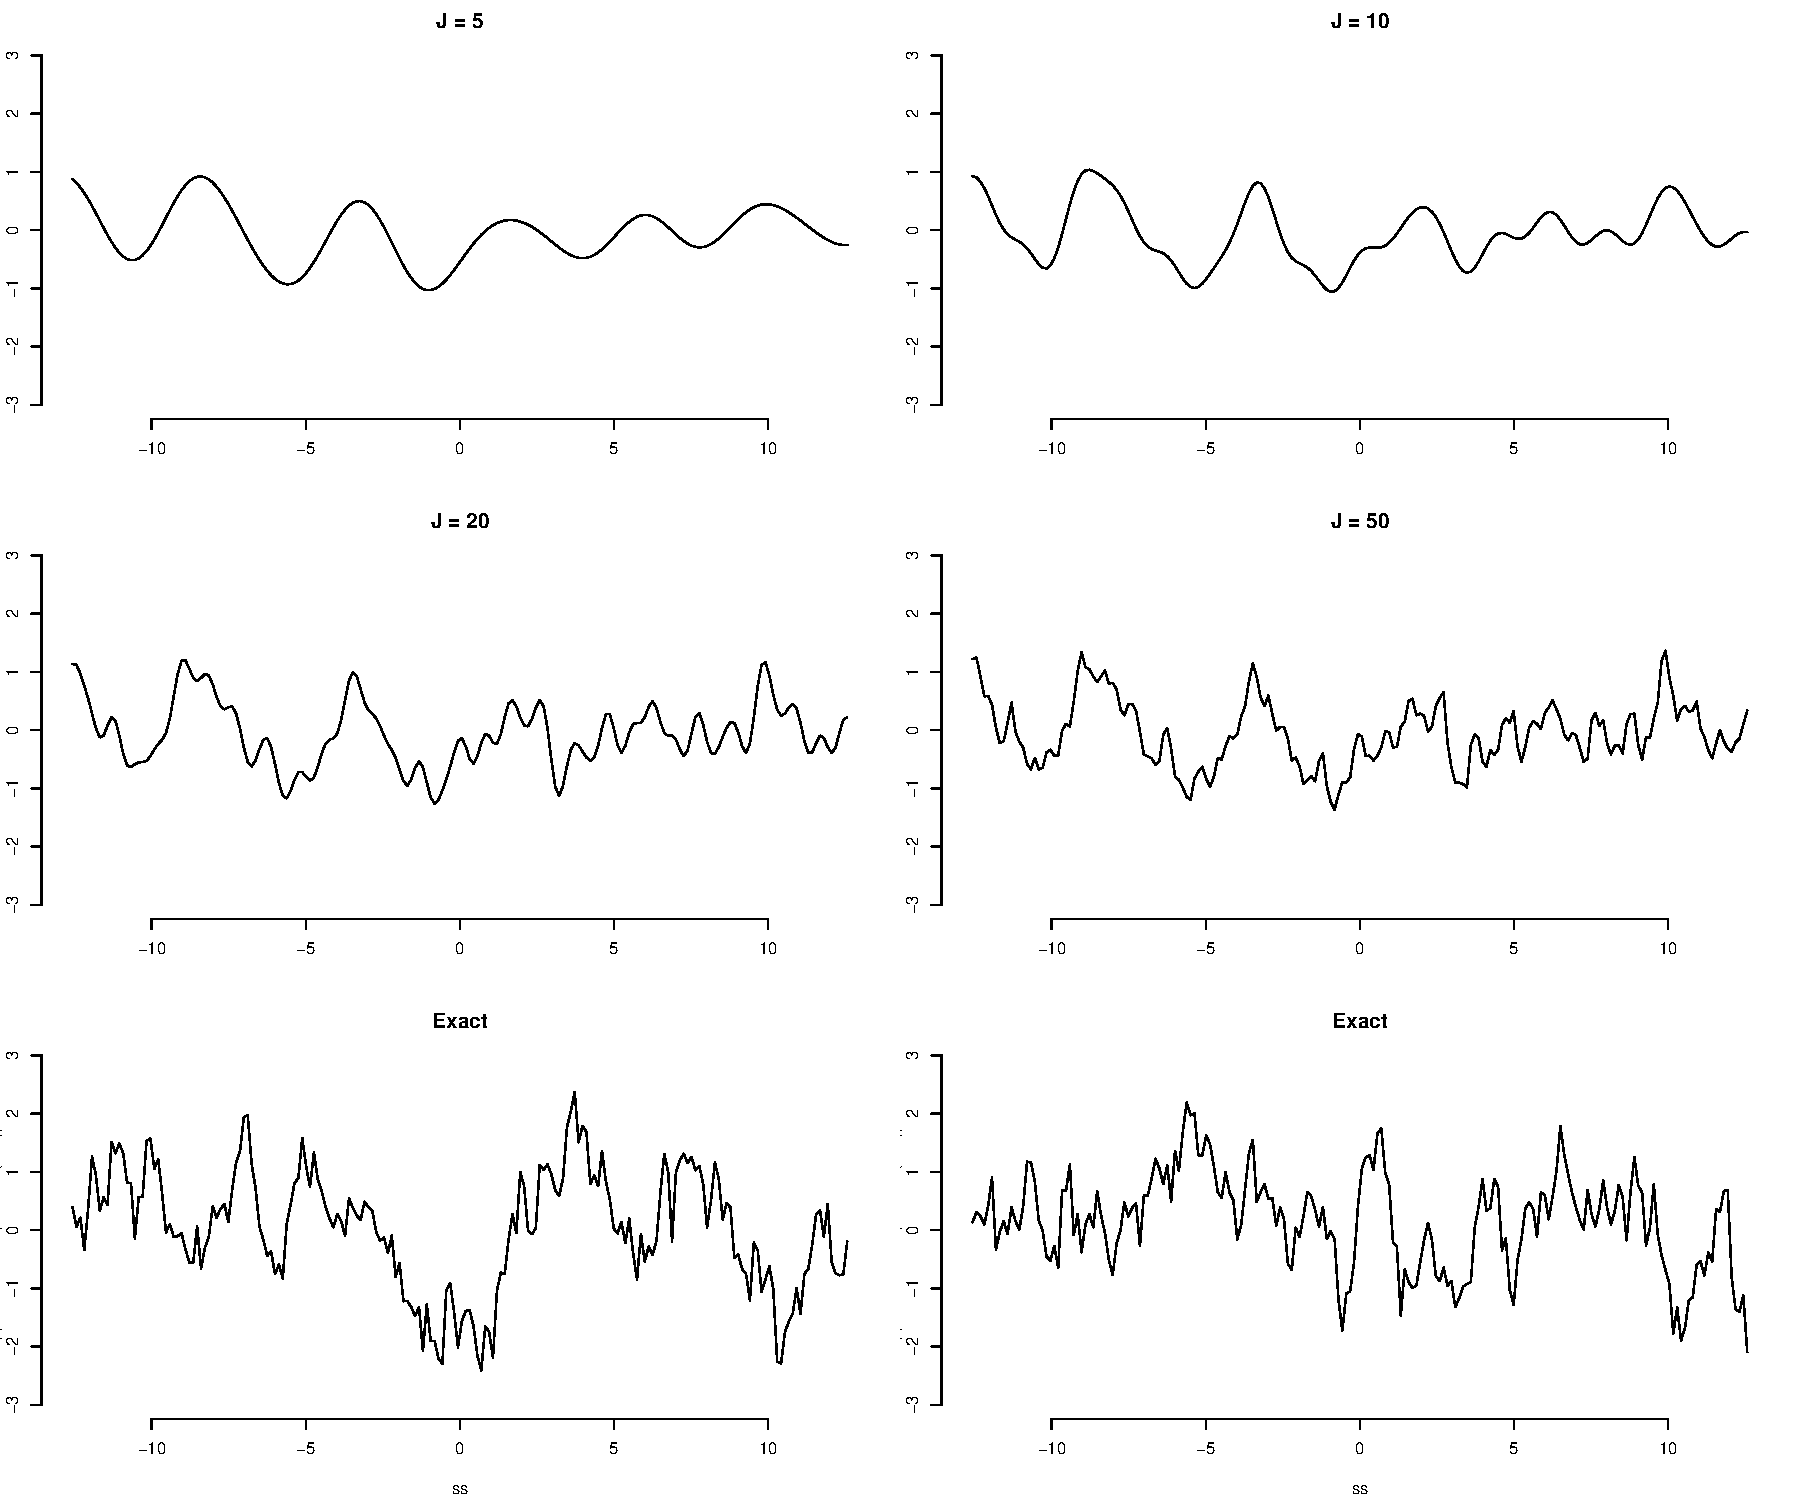
\includegraphics[scale=0.5]{figs/no3.pdf}
\end{center}

\subsection*{5. Repeat for the approximation given on Page 13 of the fifth set of slides.}

The approximation of interest is given by
\begin{align*}
\lambda_j\approx f(j\pi/(2L)), & & \psi_j(s)\approx ce^{ij\pi s/(2L)} \\
\end{align*}
where $f(k)$ is the spectrum at $k$ (and we set $c=1$). Since the exponential correlation is equivalent to the Mat{\'e}rn with $\nu=1/2$, the spectral density, for $\phi=1$, is given by
\[ f(k) = \frac{1}{(1+k^2)^{(n+1)/2}} \]
The next figure is comparable to the previous, except with this second approximation.

\begin{center}
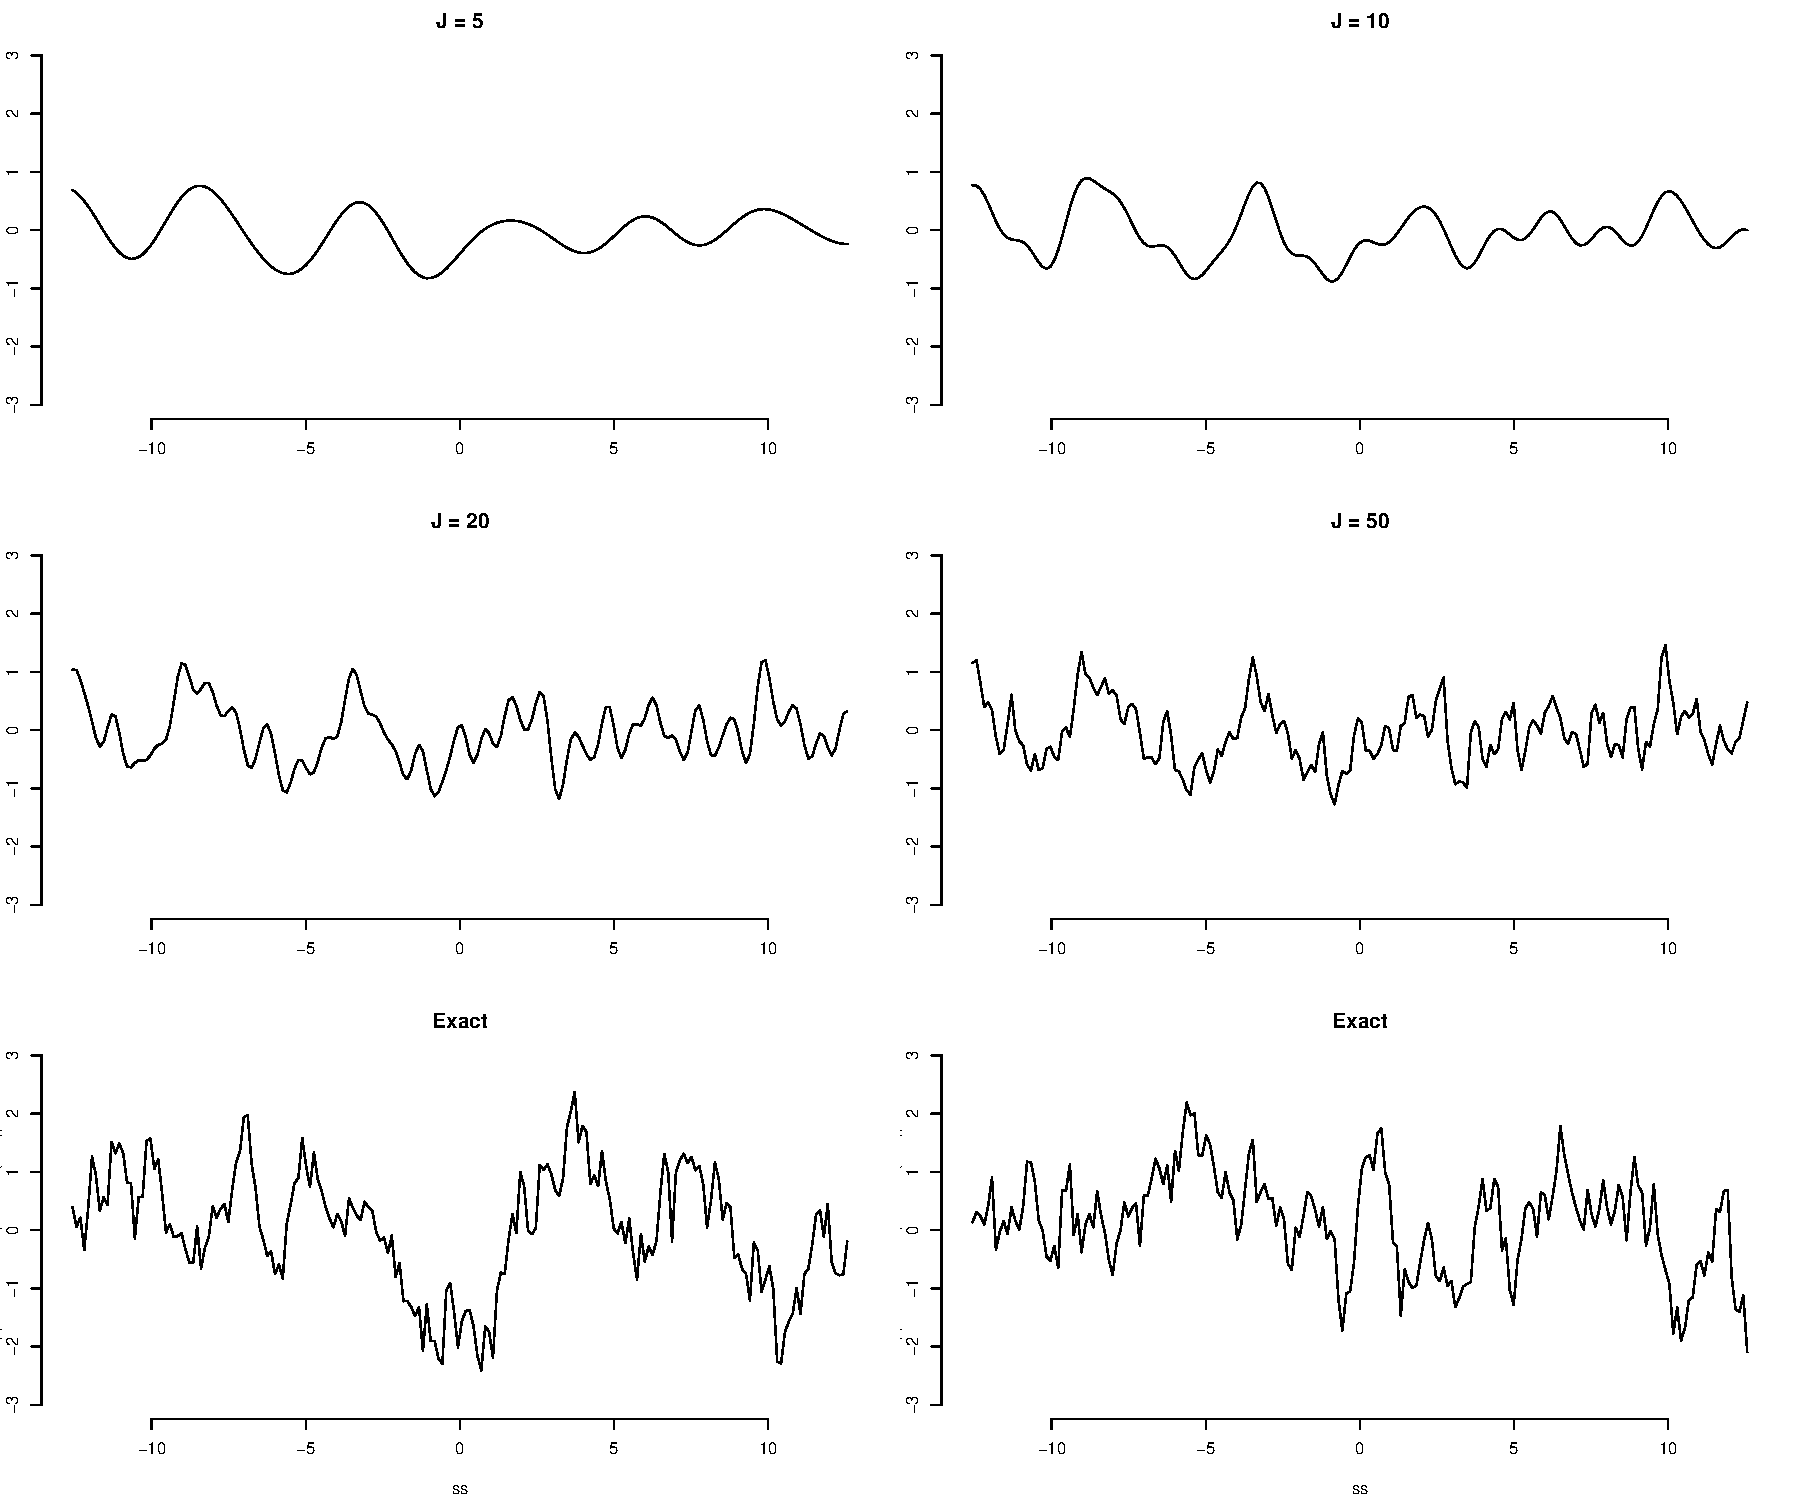
\includegraphics[scale=0.5]{figs/no4.pdf}
\end{center}

The same seed for generating the random draws was used in both problems 4 and 5. As we can see, the approximations are effectively identical. Both approaches reveal their inadequacies when $J$ is too low, but at just $J=50$, there is little distinct when obtaining realizations from the definition.

\subsection*{6. Generate 100 realizations of a univariate Gaussian process with exponential correlation with range parameter 1. Compare the empirically estimated eigenvalues and eigenfunctions to the ones given by the K-L and the approximation on Page 12.}

Empirical estimates for the eigenvalues and eigenfunctions of 100 realizations were obtained via SVD. Here, we used a cutoff at $J=50$ for the approximations. We see a substantial difference between all three eigenvalues and eigenfunctions. The eigenvalues are given in the first plot. These are scaled so the first (and largest) eigenvalue is 1 (for plotting purposes).

\begin{center}
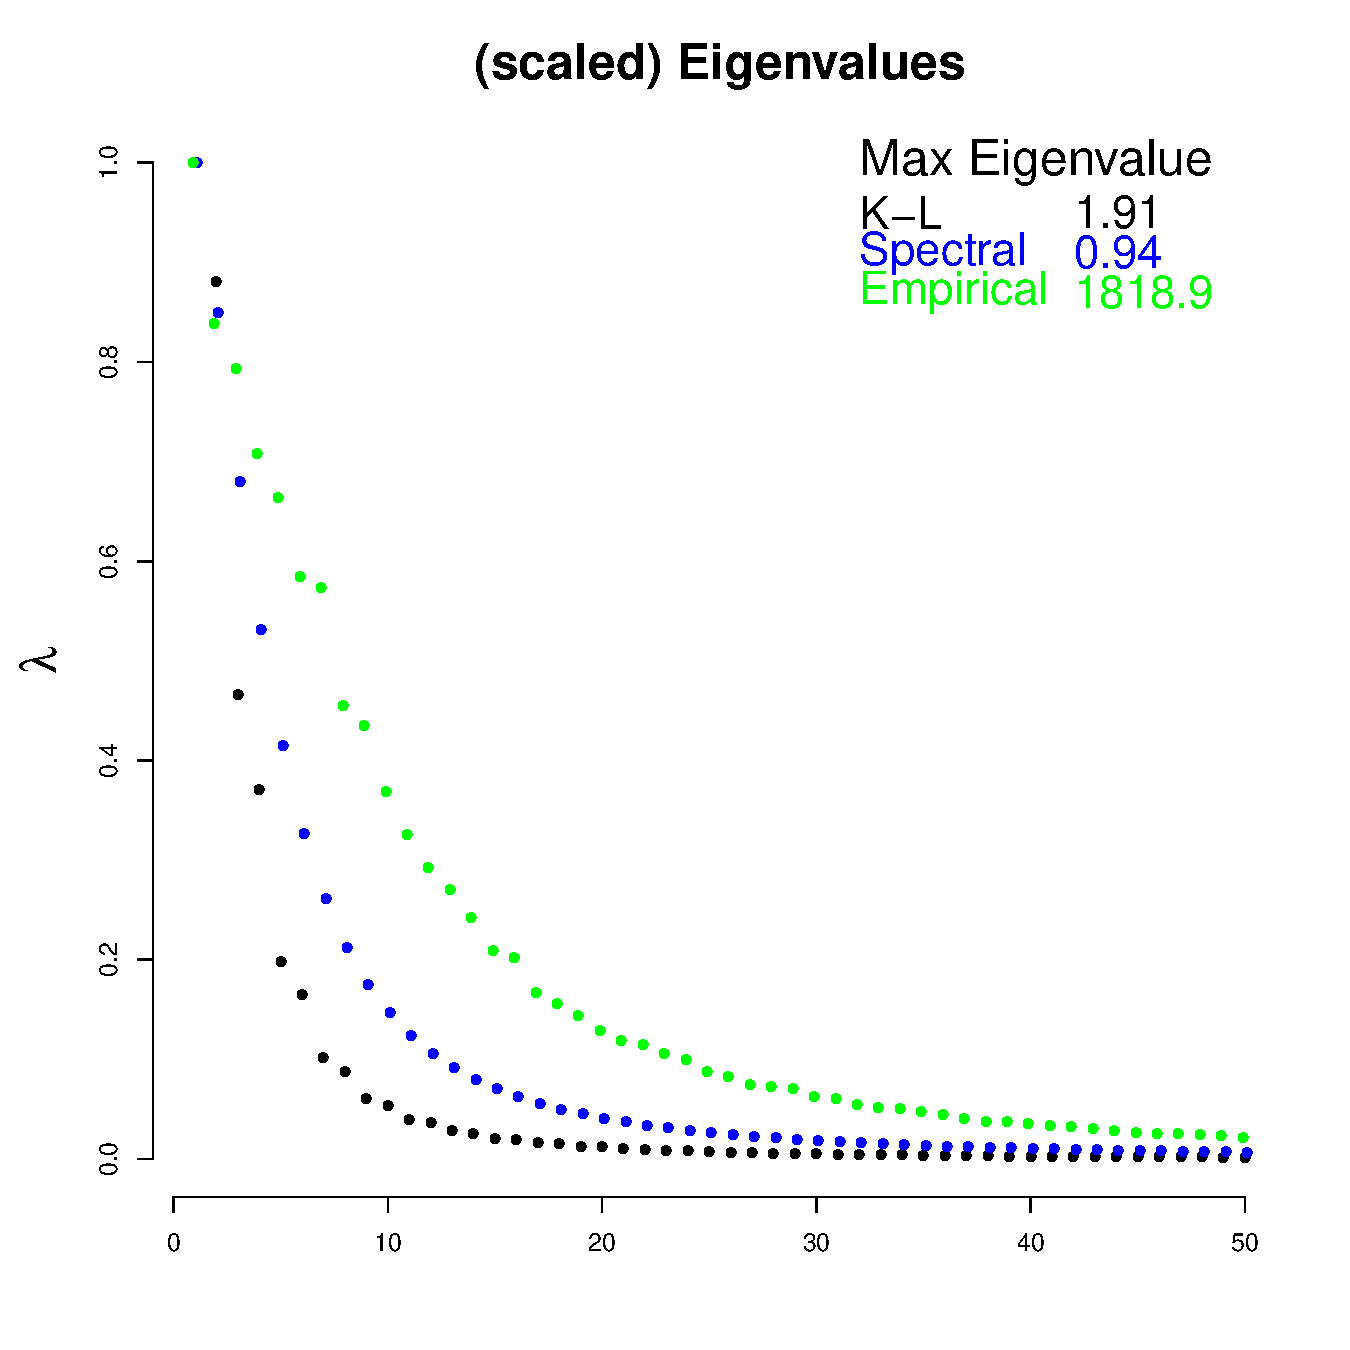
\includegraphics[scale=0.4]{figs/eval.pdf}
\end{center}

The last plot shows the eigenvectors associated with the first six eigenvalues. The are plotted against $s\in[-4\pi, 4\pi]$. The periodicity is much more evident in the approximations (perhaps due to construction). As in the first plot, black is K-L representation, blue is the approximation using the spectral density, and green is the empirical estimates from SVD.

\begin{center}
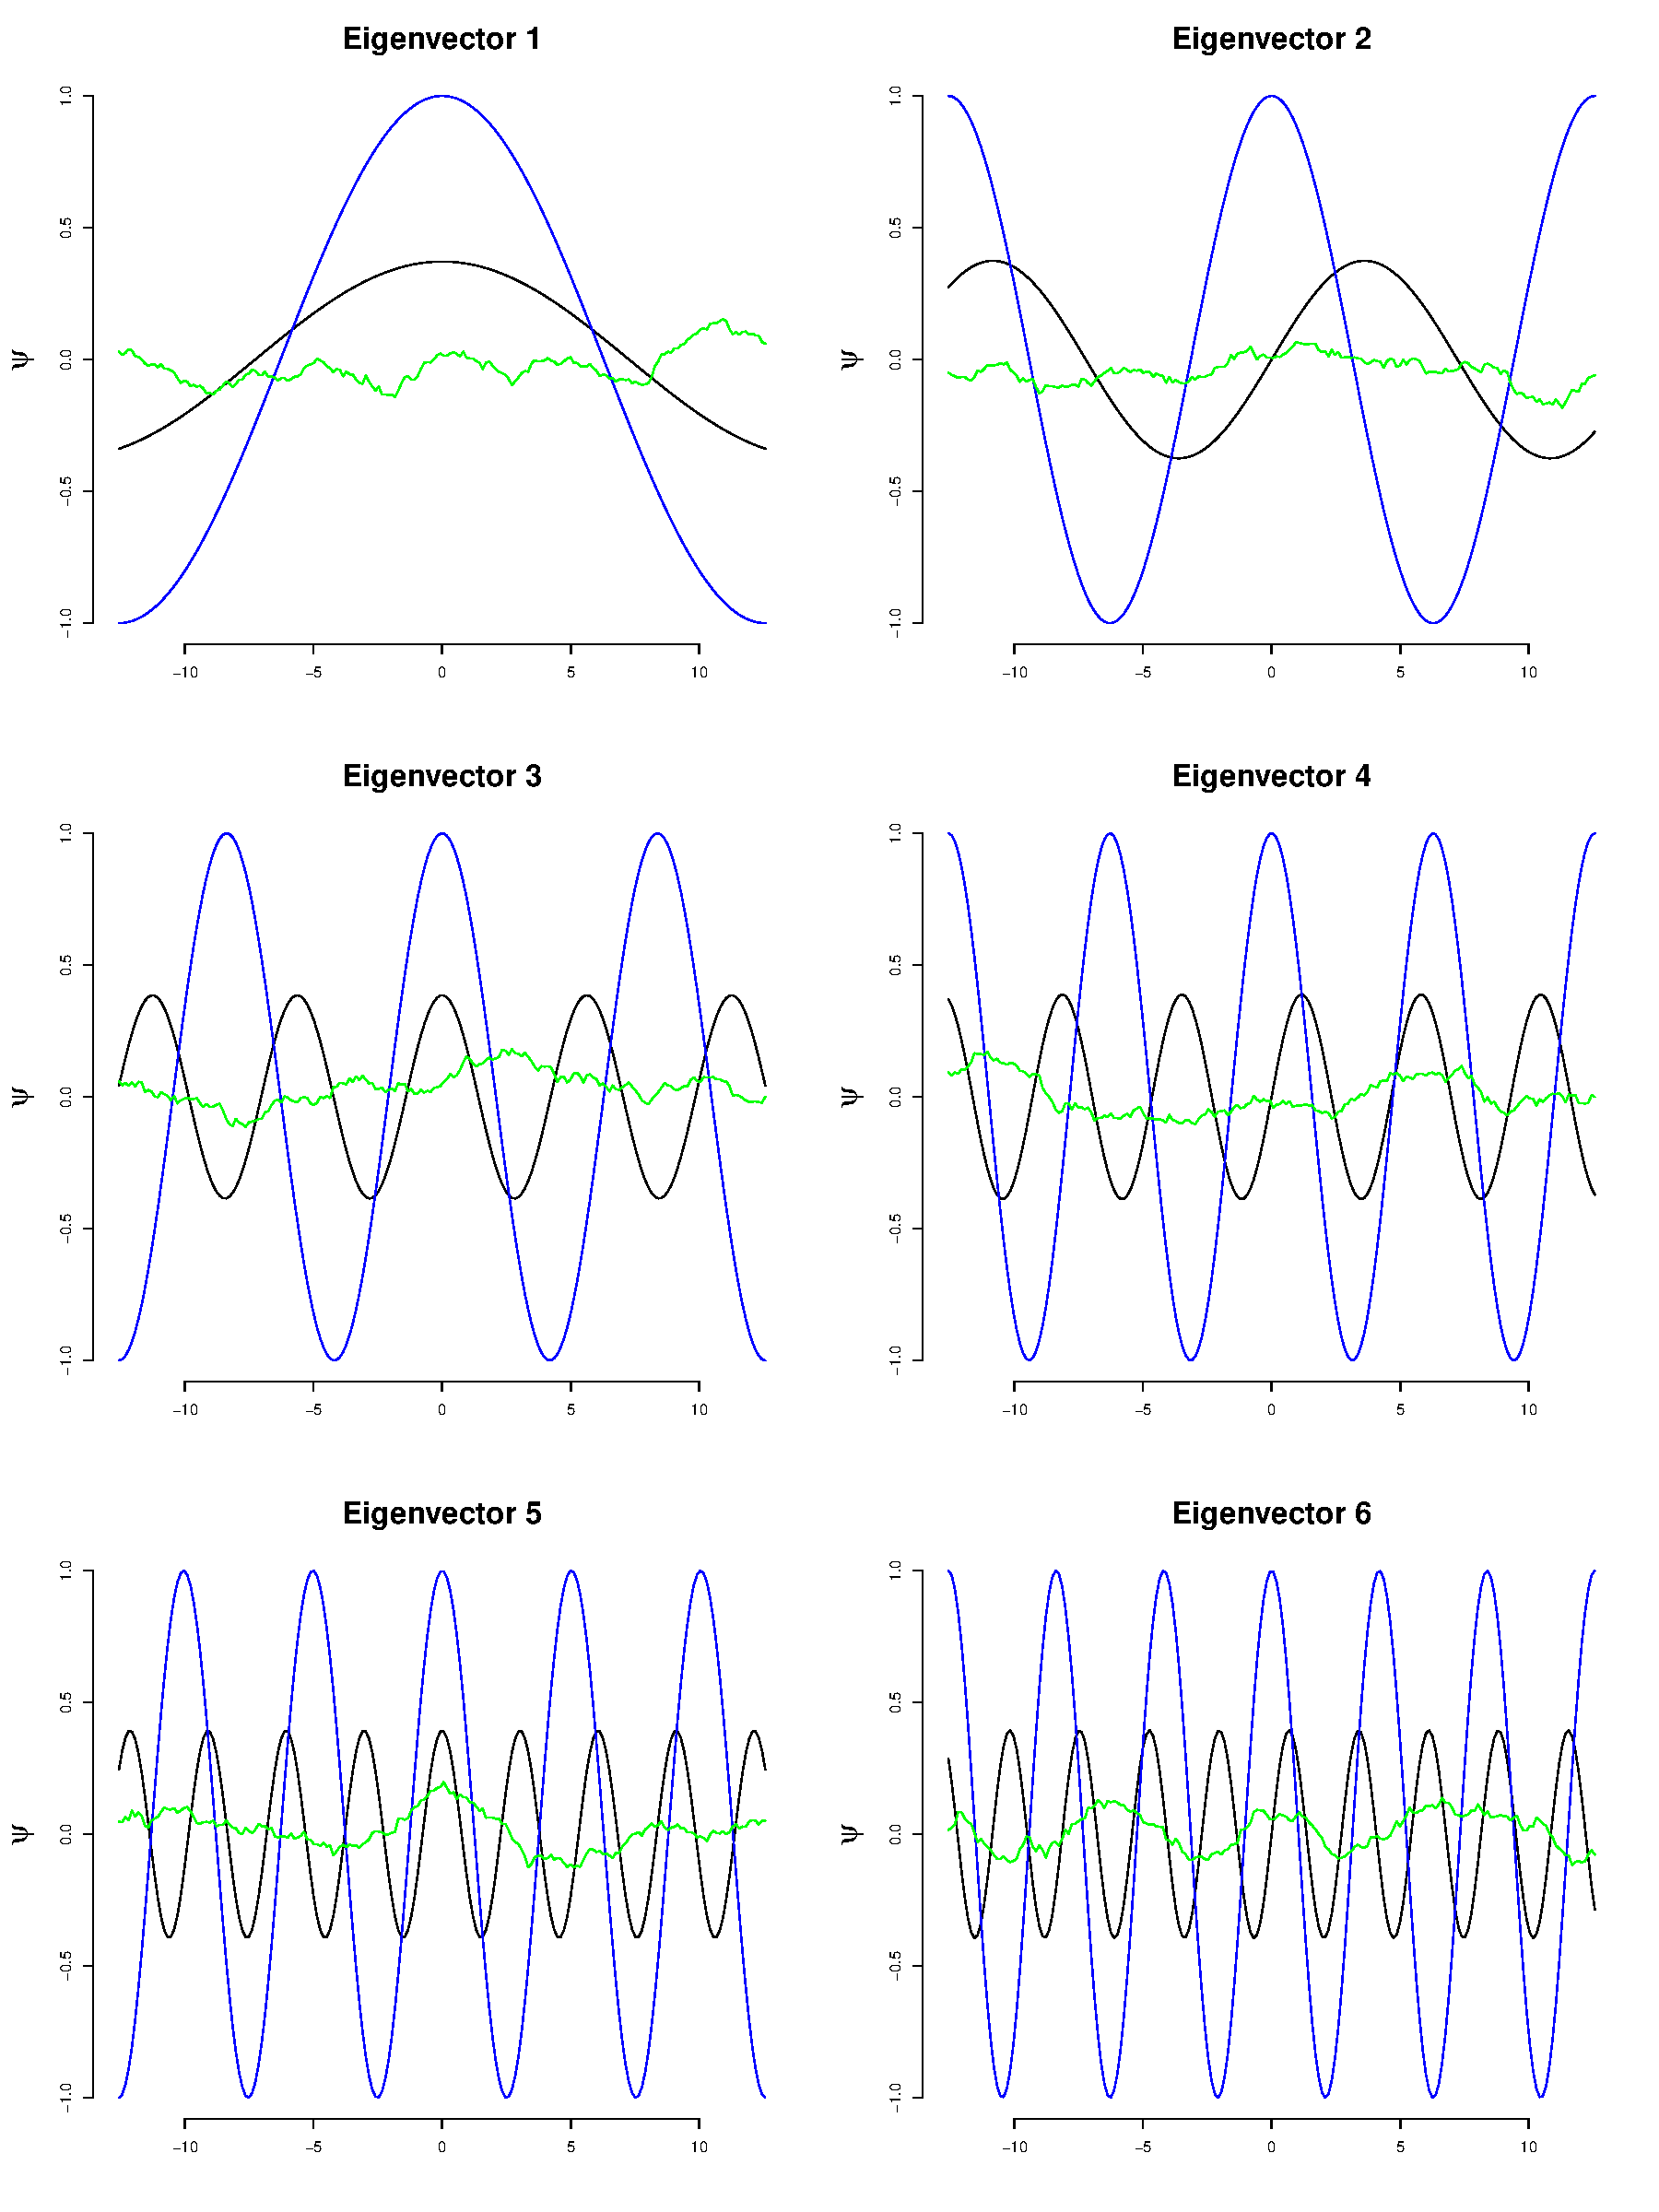
\includegraphics[scale=0.4]{figs/evec.pdf}
\end{center}

\end{document}
